\documentclass[10pt, a4paper]{article}

\usepackage{amssymb, amsmath}
\usepackage[utf8]{inputenc}
\usepackage[ngerman]{babel}
\usepackage{fancyhdr}
\usepackage{tikz}
\usepackage{fullpage}
\usepackage{graphicx}
\usepackage{alltt}
\pagestyle{fancy}
\setlength{\headheight}{12.4pt}
\setlength{\headsep}{1.5\headheight}

% 1. Person eintragen
\newcommand{\FirstAuthor}{Hasenauer}
\newcommand{\FirstAuthorFirstName}{Hannes}
\newcommand{\FirstAuthorMatnum}{**********}

% 2. Person eintragen
\newcommand{\SecAuthor}{Fritzsch}
\newcommand{\SecAuthorFirstName}{Daniel}
\newcommand{\SecAuthorMatnum}{0930754}

% 3. Person eintragen
\newcommand{\ThirdAuthor}{Temmel}
\newcommand{\ThirdAuthorFirstName}{Hans Christian}
\newcommand{\ThirdAuthorMatnum}{*********}

\newcommand{\AuthorFront}{{\normalsize
\begin{tabular}{|c|c|c|} \hline
\textbf{Nachname} & \textbf{Vorname}       & \textbf{Matrikelnummer} \\ \hline \hline
\FirstAuthor      & \FirstAuthorFirstName  & \FirstAuthorMatnum      \\ \hline
\SecAuthor        & \SecAuthorFirstName    & \SecAuthorMatnum        \\ \hline
\ThirdAuthor      & \ThirdAuthorFirstName  & \ThirdAuthorMatnum      \\ \hline
\end{tabular}}}

\author{\AuthorFront}
\newcommand{\Author}{\FirstAuthorMatnum, \SecAuthorMatnum,
                     \ThirdAuthorMatnum}

\date{} % Kein Datum angegeben
\fancyfoot{} % Seitenzahl unten nicht anzeigen

\lhead{Modern Information Systems}
\chead{\Author}
\rhead{Seite \thepage}

\title{Modern Information Systems WS 11/12}

\begin{document}

%%%%%%%%%%%%%%%%%%%%%%%%%%%%%%%%%%%%%%%%%%%%%%%%%%%%%%%%%%%%%%%%%%%%%%%%%%%%%%%%

\newcounter{ale}
\newcommand{\abc}{\item[\alph{ale})]\stepcounter{ale}}
\newenvironment{liste}{\begin{itemize}}{\end{itemize}}
\newcommand{\aliste}{\begin{liste} \setcounter{ale}{1}}
\newcommand{\zliste}{\end{liste}}
\newenvironment{abcliste}{\aliste}{\zliste}

%%%%%%%%%%%%%%%%%%%%%%%%%%%%%%%%%%%%%%%%%%%%%%%%%%%%%%%%%%%%%%%%%%%%%%%%%%%%%%%%

\maketitle
\thispagestyle{fancy}

%%%%%%%%%%%%%%%%%%%%%%%%%%%%%%%%%%%%%%%%%%%%%%%%%%%%%%%%%%%%%%%%%%%%%%%%%%%%%%%%

\tableofcontents
\pagebreak

\section{Database Schema}

\subsection{Entity-Relationship Diagram}
\begin{figure}[htb]
	\centering
	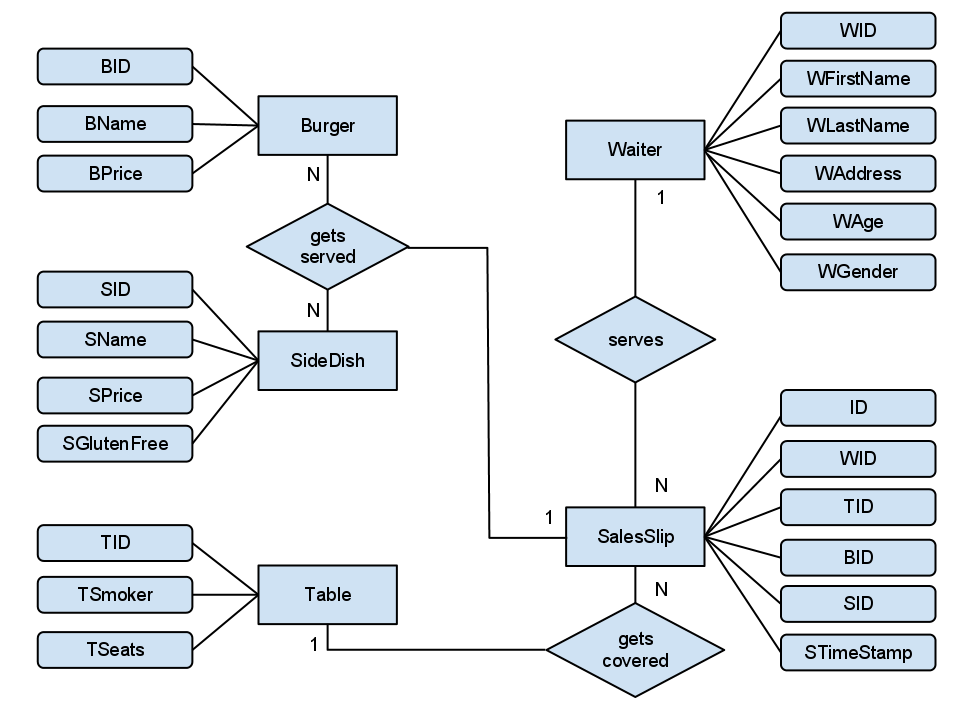
\includegraphics[scale=0.49]{fig/entity_relationship_diagram.png}
	\caption{Entity-Relationship Diagram}
\end{figure}

\subsection{Domains}

\end{document}